\section{Durchführung}
\label{sec:Versuchsaufbau und Durchführung}
\begin{figure}[H]
    \centering
    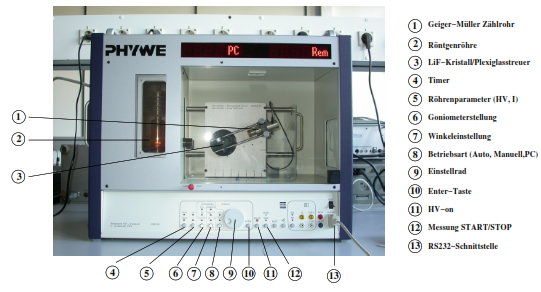
\includegraphics{Röntgenröhre.png}
    \caption{Röntgenröhre.}
    \label{fig:Röntgenröhre}
  \end{figure} 
  \paragraph{}
In \autoref{fig:Röntgenröhre} ist der Abbau der Röntgengerät zu sehen. 

Das Emissionspektrum (Aufgabe 1) und die Transmission $T(\lambda)$ des Aluminium-Absorbers werden mit dem Rechner gemessen.
Die Compton-Wellenlänge wird durch die manuelle Bedienung bestimmt. 
Das Experiment wirde den PC gesteuert. 
Die gemessenen Zählrate erscheint in der oberen Anzeigeleiste des Röntgengerätes.

Bei dem ganzem Versuch werden Beschleunigungsspannung auf 35kV und Emmusionsstrom auf 1mA gestellt. LiF-Kristall wird in die Halterung gesteckt.
\paragraph{}
1. Aufnahme eines Emissionspektrums der Kupfer Röntgenröhre

Dafür werden eine 2mm Blende und einen LiF-Kristall verwendet. 
Das Röntgenspektrum (Beugungsordnung \(n=1 \)) wird in Schritten von \(\Delta\alpha=0,1° \) und einer Integrationszeit von  \(t=10 \,s \) gemessen.
\paragraph{}
2. Bestimmung der Transmission als Funktion der Wellenlänge und die Compton-Wellenlänge

 a. Die Transmission $T(\lambda)$ des Aluminium-Absorbers wird für die Bestimmung der Compton-Wellenlänge aufgenommen.
 Der Al-Absorber wird vor die 2mm Blende gesetzt. 
 In Schritten von \(\Delta\alpha=0,1° \) werden $N_{Al}$ mit Absorber und $N_{0}$ ohne Absorber als Funktion des Kristallwinkelns in einem Bereich von \(7° \leq \alpha \leq 10°\) gemessen. (Messzeit \(t=200 \,s \))

 Die Transmission \(T= I_{Al}/ I_0\) wird berechnet durch
 \begin{equation}
  I= \frac{N}{1-\tau \cdot N}
  \end{equation}
  wobei die Totzeit \(\tau=90 \,\mu s \) ist.
 
  b. Ab diesem Teil des Versuches wird die manuelle Messung durchgeführt.
  Der Versuch wird umgebaut: die 2mm Blende wird durch 5mm Blende eingesetzt und der LiF-Kristall wird durch einen Plexiglas-Streuer ausgetauscht. 
  Der Kristall wird auf 45° und das Geider-Müller Zahlrohr wird auf 90° gestellt (siehe \autoref{fig:Experimenteller Aufbau}).
 Die Intensität $I_0$ der Cu-Röhre wird gemessen.
\begin{figure}[H]
    \centering
    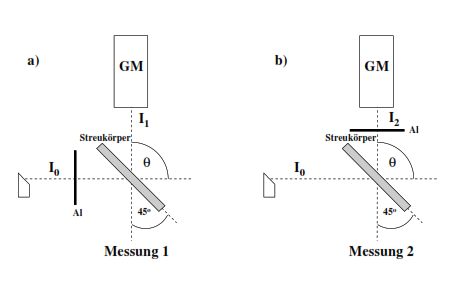
\includegraphics{Experimenteller Aufbau.png}
    \caption{Experimenteller Aufbau.}
    \label{fig:Experimenteller Aufbau}
  \end{figure} 
  c. Bestimmung der Compton-Wellenlänge $\lambda_c$
 
Zwei unabhängige Messungen werden durchgeführt.
Die Transmission \(T= I_1 / I_0\) (\autoref{fig:Experimenteller Aufbau} links) der ungestreuten Röntgenstrahlung und die Transmission \(T= I_2 / I_0\) (\autoref{fig:Experimenteller Aufbau} rechts) der gestreuten Röntgenstrahlung werden bestimmt. 
(Messzeit \(t=300 \,s\))

Die Messungen werden 5 mal wiederholt.
\cite{AL}
\newpage